\section{Data Pre-processing}
The dataset utilized in this study is derived from a CSV file containing comprehensive specifications of Intel CPUs. This dataset serves as the foundation for our analysis, providing detailed information on various CPU features that are essential for understanding clock speed trends. In this section, we describe the dataset's structure, contents, and the relevance of its attributes to our study.

\subsection{Dataset Overview}
The CSV file comprises numerous rows, each representing an individual Intel CPU model. Each row contains multiple attributes describing the specifications and characteristics of the CPU. The dataset encompasses a diverse range of CPU models across different series, generations, and intended applications (e.g., consumer desktops, laptops, server-grade CPUs), ensuring a comprehensive coverage of CPU types and their respective attributes.

\subsection{Data Relevance and Usefulness}
The following attributes from the dataset are particularly relevant for analyzing CPU clock speeds:

\begin{itemize}
    \item \textbf{Processor\_Base\_Frequency}: This attribute represents the base clock speed of the CPU, measured in gigahertz (GHz). Higher base frequencies generally indicate faster processing capabilities and overall performance.
    \item \textbf{Max\_Turbo\_Frequency}: Many modern CPUs support Turbo Boost technology, which dynamically increases the clock speed under certain conditions. This attribute specifies the maximum Turbo Boost frequency achievable by the CPU, providing insights into its potential performance capabilities.
    \item \textbf{nb\_of\_Cores}: The number of cores in a CPU impacts its ability to handle multiple tasks simultaneously. CPUs with more cores can potentially support higher clock speeds under optimal conditions, affecting overall performance trends.
    \item \textbf{nb\_of\_Threads}: This attribute represents the number of threads supported by the CPU, which is often influenced by technologies like Intel's Hyper-Threading. A higher number of threads can contribute to better resource utilization and potentially higher effective clock speeds for certain workloads.
    \item \textbf{TDP (Thermal Design Power)}: The TDP indicates the maximum amount of heat the CPU cooling system needs to dissipate. This attribute is closely related to the CPU's power consumption and thermal characteristics, which can impact clock speed potential and performance.
    \item \textbf{Lithography}: This attribute refers to the manufacturing process node (e.g., 14nm, 10nm) used in producing the CPU. Advancements in manufacturing processes can lead to higher clock speeds and improved efficiency in newer CPU generations.
\end{itemize}

Our objective is to analyze historical trends in CPU clock speeds using these attributes. Understanding how clock speeds have evolved across different CPU generations, architectural improvements, and technological shifts is crucial for identifying patterns and making informed predictions. By focusing on these critical attributes, we aim to uncover insights into the factors driving CPU clock speed improvements and contributing to the overall technological progress in CPU development.

\subsection{Load Data}
\begin{lstlisting}[language=R]
    # Importing data 
    intel_cpu <- read.csv ("~/Downloads/archive/Intel_CPUs.csv")
\end{lstlisting}

This line of R code is used to import a dataset from a Comma-Separated Values (CSV) file into the R environment.
The \texttt{read.csv()} function is a built-in function in R that reads a CSV file and creates a data frame object from its contents. A data frame is a two-dimensional tabular data structure in \texttt{R}, where each column represents a variable, and each row represents an observation.\\

In this specific code:
"\textbf{$\sim$/Downloads/archive/Intel\_CPUs.csv}" is the file path that specifies the location and name of the CSV file to be imported, \texttt{intel\_cpu} is the name assigned to the data frame object that will store the imported data.\\

After executing this line of code, the contents of the "\textbf{Intel\_CPUs.csv}" file will be read and stored in the \texttt{intel\_cpu} data frame within the \texttt{R} environment. The data frame will have the same structure as the CSV file, with columns representing variables and rows representing observations.

\subsection{Explore Data}
\begin{lstlisting}[language=R]
    # The head () function is used to preview the first 
    # few rows of the data frame
    head (intel_cpu)
\end{lstlisting}

This line calls the \texttt{head()} function and passes the \texttt{intel\_cpu} data frame as an argument. By default, the \texttt{head()} function prints the first \textit{six} rows of the given data frame or matrix.\\

The \texttt{head()} function is a valuable tool for data exploration and validation, especially when working with large datasets. By previewing the initial rows, you can quickly assess the structure of the data, check the column names, and ensure that the data has been imported correctly.\\

Inspecting the first few rows can reveal potential issues or anomalies in the data, such as missing values, incorrect data types, or unexpected values. It also provides an initial glimpse into the content and format of the data, which can inform subsequent data cleaning, transformation, or analysis steps

\begin{figure}[H]
    \centering
    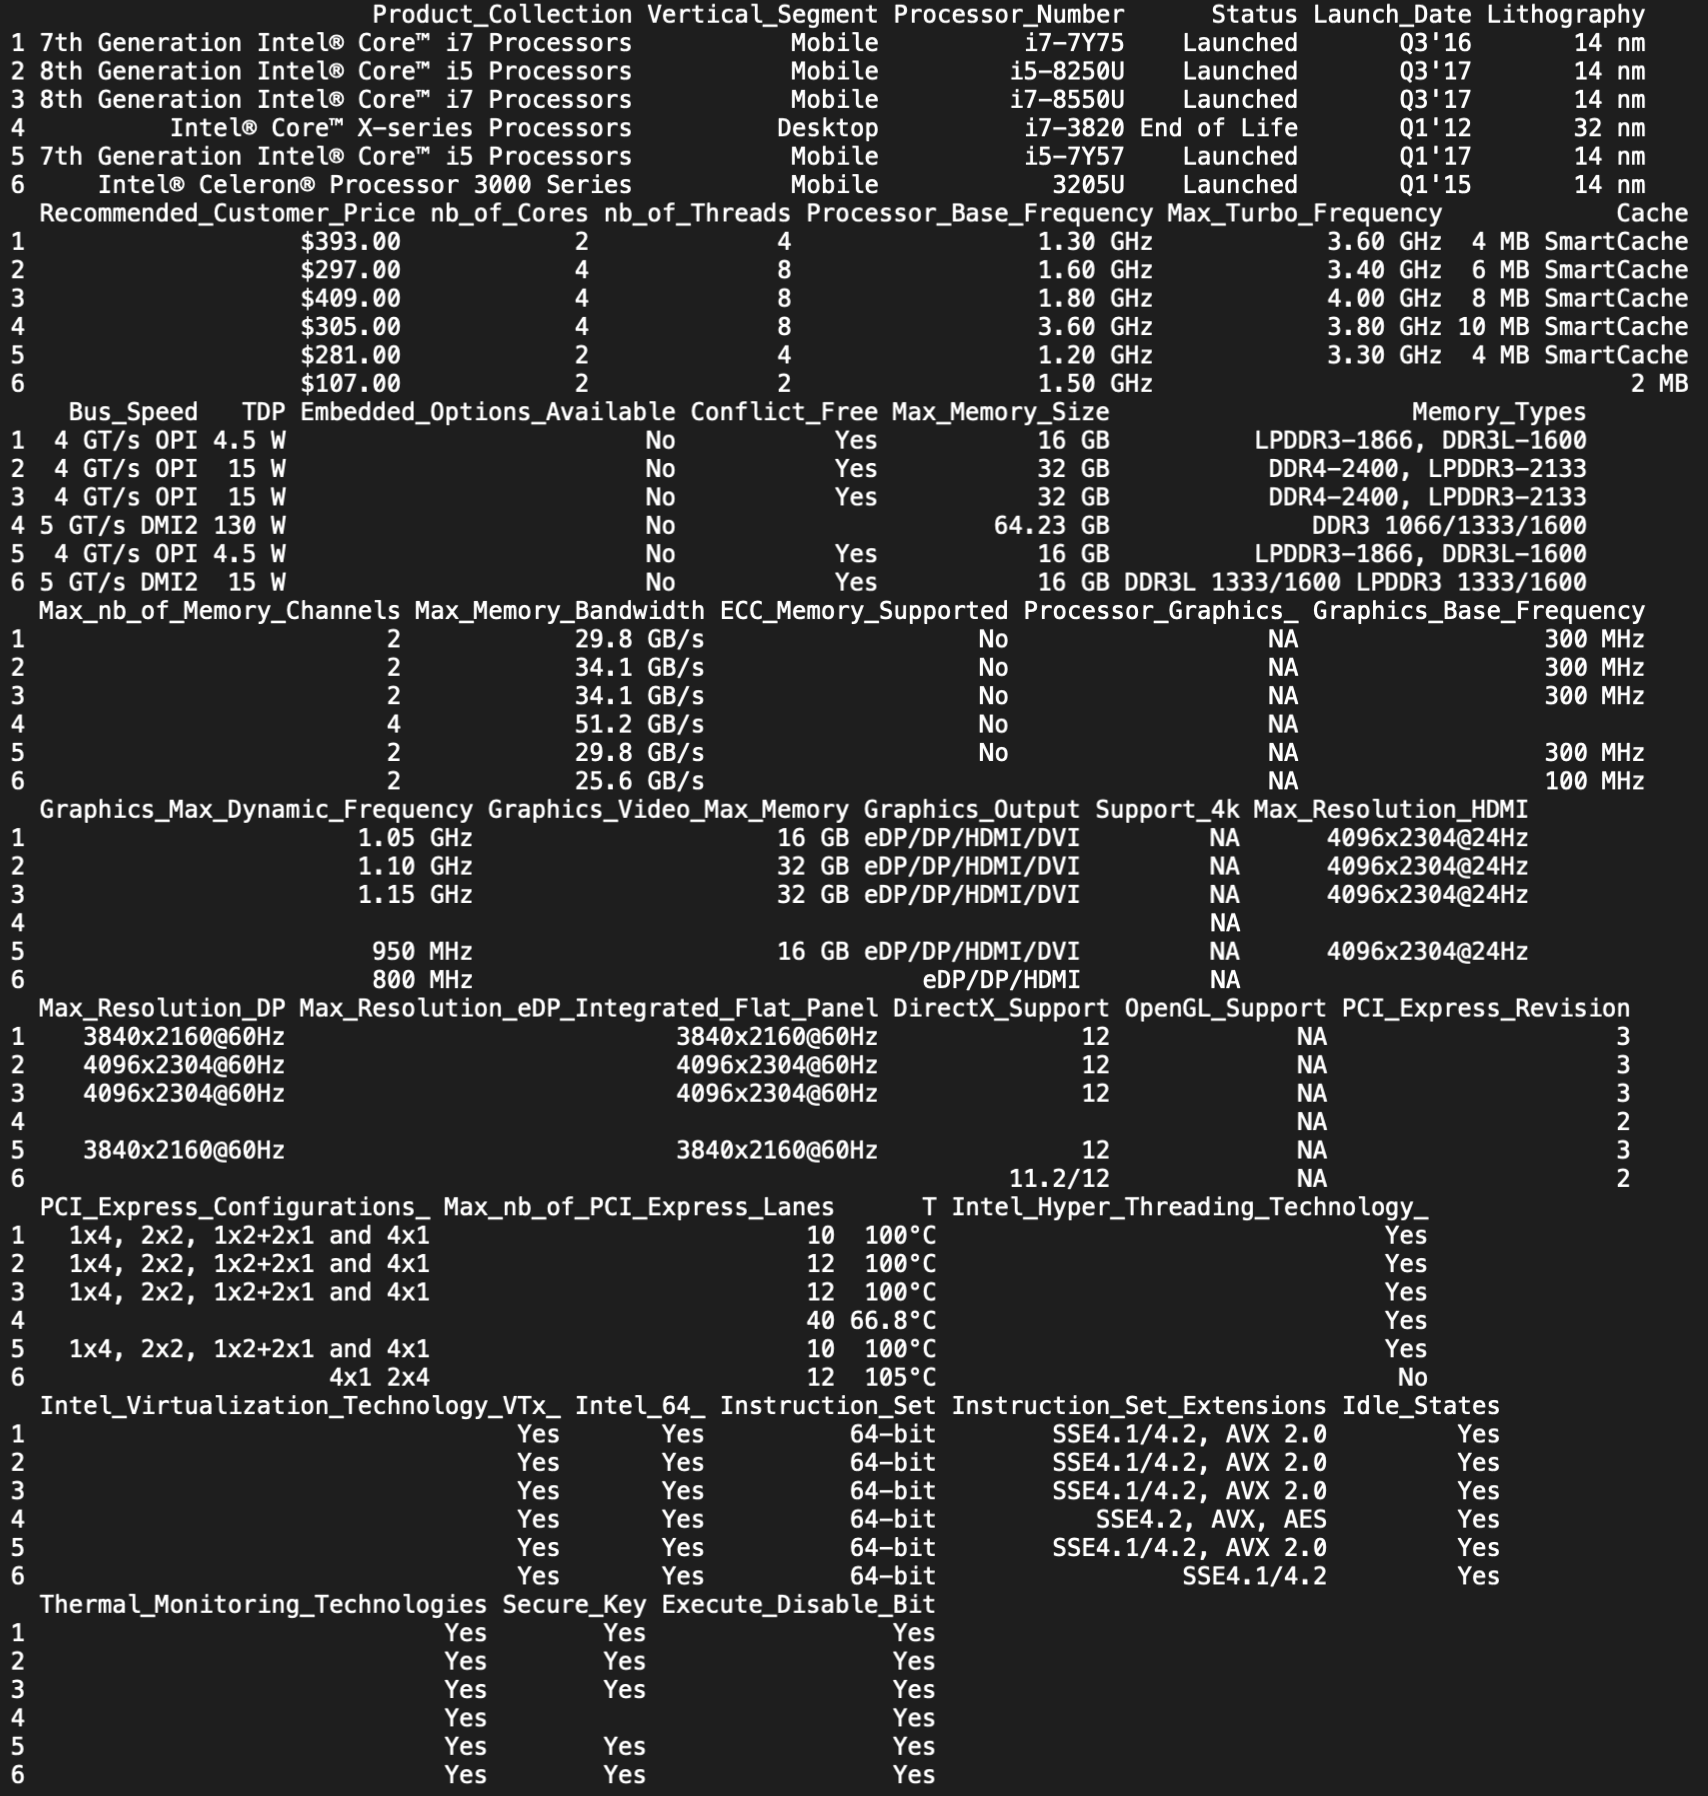
\includegraphics[width=14cm]{graphics/head.png}
    \caption*{Console output of \texttt{head(intel\_cpu)}}
\end{figure}

By executing \texttt{head(intel\_cpu)}, the output will display the first \textit{six} rows of the \texttt{intel\_cpu} data frame, allowing you to visually inspect the data and make informed decisions about the next steps in the data analysis workflow.

\newpage

\begin{lstlisting}[language=R]
    # Summary statistics
    summary (intel_cpu)
\end{lstlisting}

This code snippet is used to obtain summary statistics for the dataset stored in \texttt{intel\_cpu}.\\

The \texttt{summary ()} function in \texttt{R} is a versatile tool that provides a consise summary of the data, depending on the type of input it receives.

\begin{figure}[H]
    \centering
    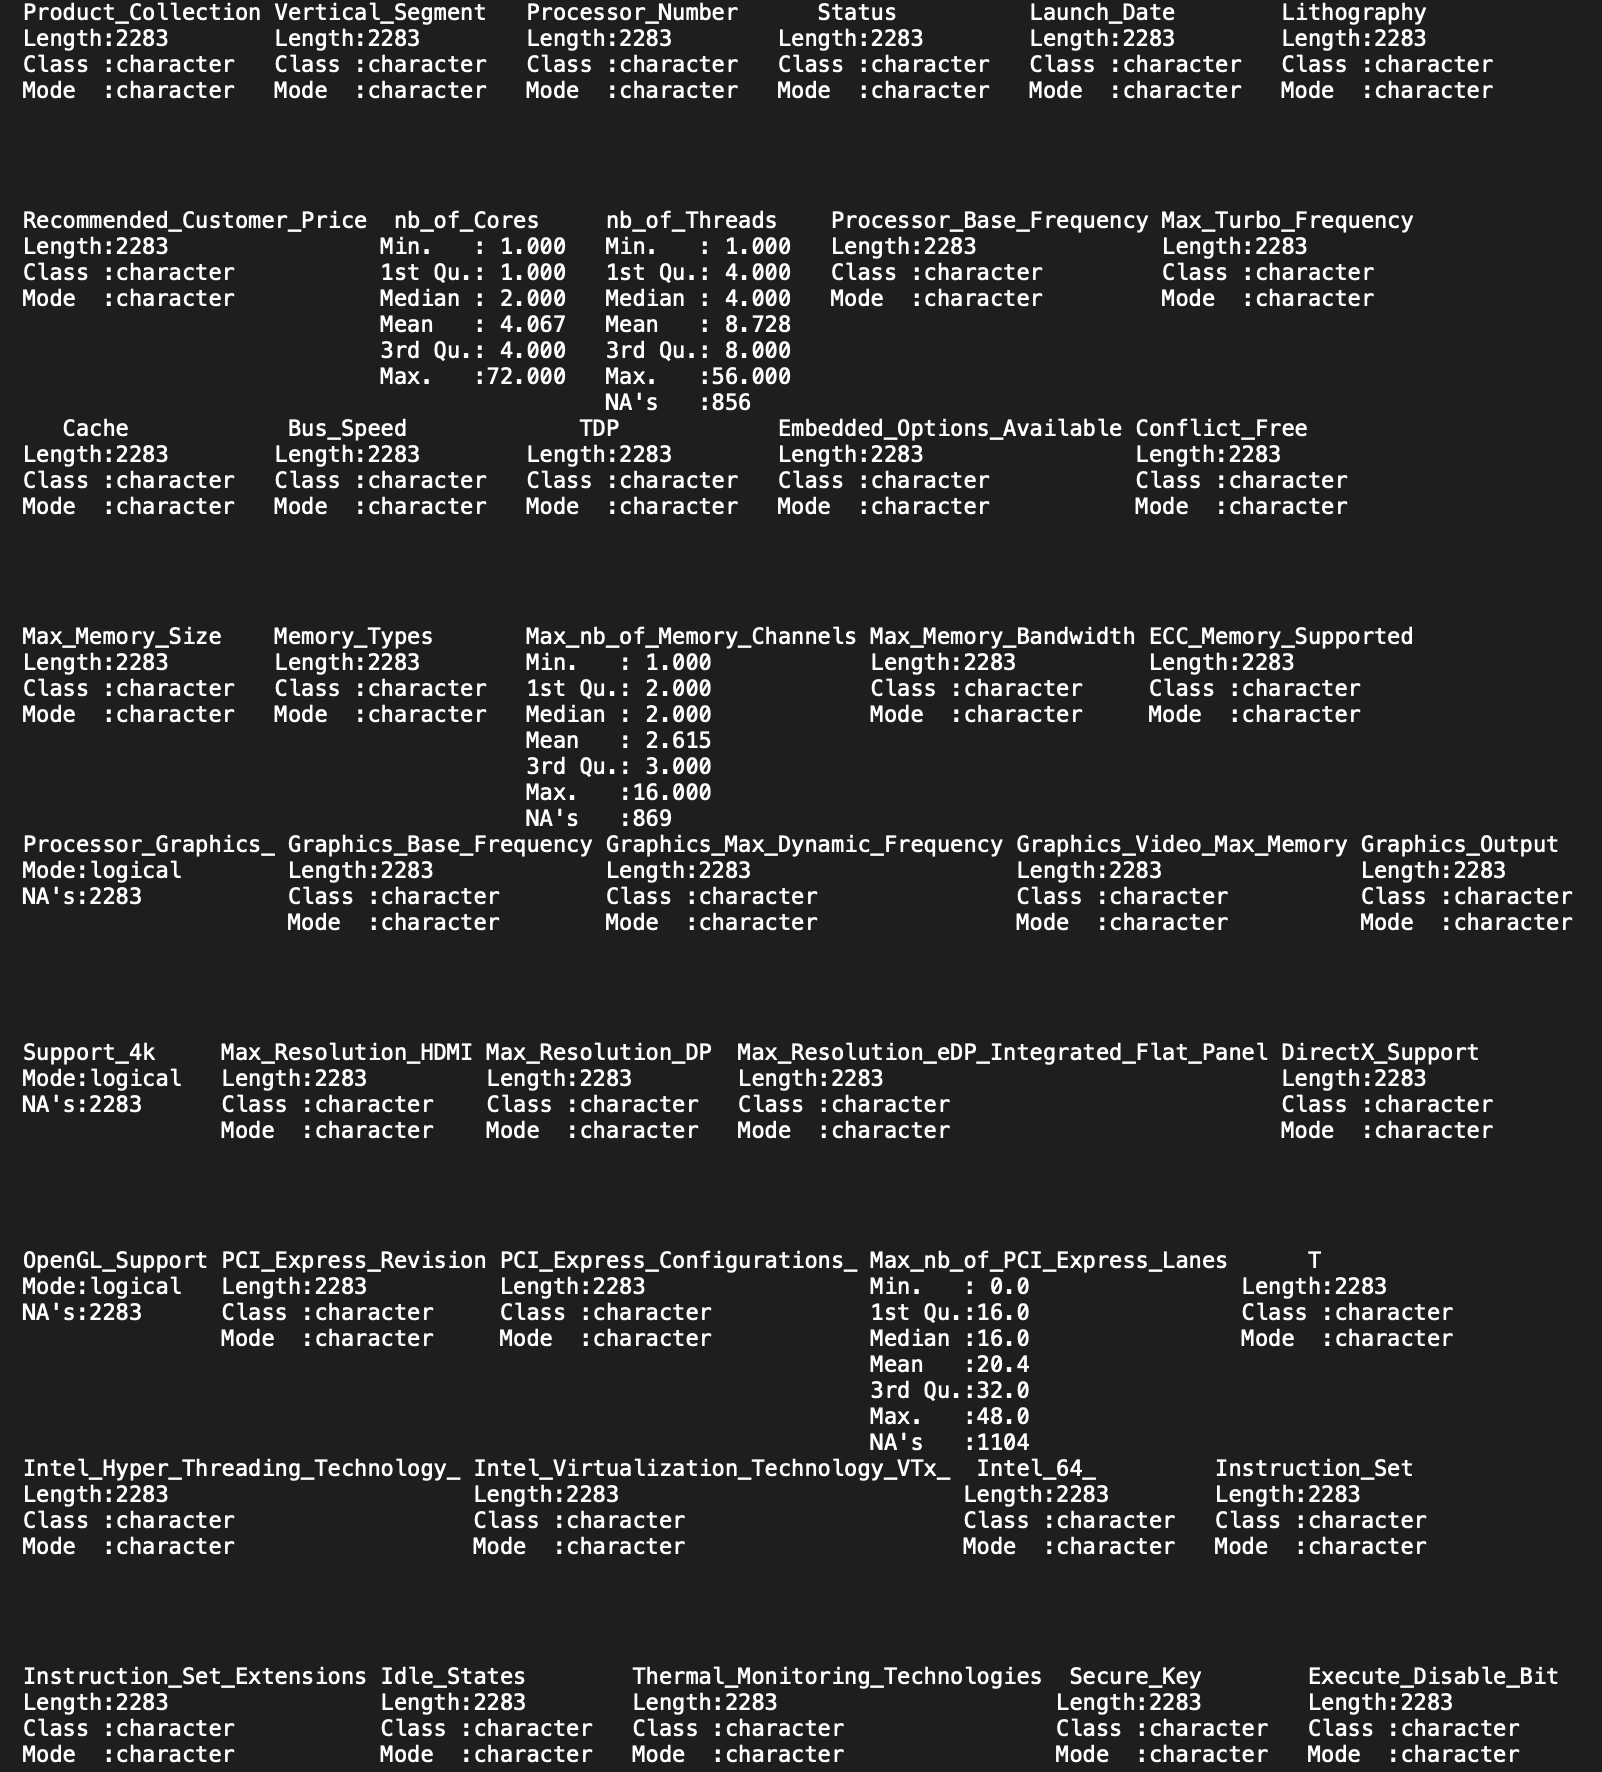
\includegraphics[width=14cm]{graphics/summary.png}
    \caption*{Console output of \texttt{summary(intel\_cpu)}}
\end{figure}

\subsection{Handle Missing Values}

\subsection{Handle Outliers}

\subsection{Feature Scaling/Normalization}

\newpage